\documentclass[a4paper,10pt]{article}
\usepackage{epsfig}
\usepackage{float}
\usepackage{slashbox}
\usepackage{wrapfig}
\usepackage{tabularx,ragged2e,booktabs,caption}
\usepackage{solutions}
\usepackage{amsmath,amssymb}
\DeclareRobustCommand{\bbone}{\text{\usefont{U}{bbold}{m}{n}1}}
\DeclareMathOperator{\EX}{\mathbb{E}}% expected value
\begin{document}
%%% fill in your team name and each student's name:
\frontpage{Hadamard}{Leonardo Romor, Maurice Frank, Simone Astarita, XinYu Fu, Yije Zhang}{1}

%%%%%%%%%%%%%%%%%%%%%%%%%%%%%%%%%%%%%%%%%%%%%%%%%%%%%%%%%%%%%%%%%%%%%%%%%%

\begin{nproblem}{7}{Two coins and a die}
You have two (fair) coins and a (fair) 4-sided die with outcomes $\{1,2,3,4\}$. Let $X$ be the number of heads after flipping the two coins and let $Y$ be the result of rolling the die. Let $Z$ be the average of $X$ and $Y$.
\end{nproblem}

\begin{subproblem}{2}
What is the distribution $P_Z$ of $Z$?
\end{subproblem}

\begin{solution}
We can first write down $P_X$ in \autoref{table:1} and $P_Y$ in \autoref{table:2}. Then, it is easy to get the distribution of $Z$ by simple counting. $P_Z$ is shown in \autoref{table:3}.

\begin{table}[ht]
\centering
\caption{Distribution of $X$}
\begin{tabular}{c c c c}
\hline
$X$ & 0 & 1 & 2 \\ [0.5ex]
\hline
P($X$)& $\frac{1}{4}$ & $\frac{1}{2}$ & $\frac{1}{4}$ \\
\hline
\end{tabular}
\label{table:1}
\end{table}

\begin{table}[ht]
\caption{Distribution of $Y$}
\centering
\begin{tabular}{c c c c c}
\hline
$Y$ & 1 & 2 & 3 & 4 \\ [0.5ex]
\hline
P($Y$)& $\frac{1}{4}$ & $\frac{1}{4}$ & $\frac{1}{4}$ & $\frac{1}{4}$\\
\hline
\end{tabular}
\label{table:2}
\end{table}

\begin{table}[ht]
\caption{Distribution of $Z$}
\centering
\begin{tabular}{c c c c c c c}
\hline
$Z$ & $\frac{1}{2}$ & 1 & $\frac{3}{2}$ & 2 & $\frac{5}{2}$ & 3\\ [0.5ex]
\hline
P($Z$) & $\frac{1}{16}$ & $\frac{3}{16}$ & $\frac{1}{4}$ & $\frac{1}{4}$ & $\frac{3}{16}$ & $\frac{1}{16}$\\
\hline
\end{tabular}
\label{table:3}
\end{table}
\end{solution}


\begin{subproblem}{3}
Compute the variances of $X$, $Y$ and $Z$.
\end{subproblem}

\begin{solution}
Just apply the definition of variance, easy to get:
    \begin{align}
        \mathop{{}\mathbb{E}}(X) &= 0 \times \frac{1}{4} + 1 \times \frac{1}{2} + 2 \times \frac{1}{4} = 1\\
        Var(X) &= (0-1)^{2} \times \frac{1}{4} + (1-1)^{2} \times \frac{1}{2} + (2-1)^{2} \times \frac{1}{4} = \frac{1}{2}\\
        \mathop{{}\mathbb{E}}(Y) &= 1 \times \frac{1}{4} + 2 \times \frac{1}{4} + 3 \times \frac{1}{4} + 4 \times \frac{1}{4} = \frac{5}{2} \\
        Var(Y) &= (1-\frac{5}{2})^{2} \times \frac{1}{4} + (2-\frac{5}{2})^{2} \times \frac{1}{4} + (3-\frac{5}{2})^{2} \times \frac{1}{4} + (4-\frac{5}{2})^{2} \times \frac{1}{4} = \frac{5}{4} \\
        \mathop{{}\mathbb{E}}(Z) &= \frac{1}{2} \times \frac{1}{16} + 1 \times \frac{3}{16} + \frac{3}{2} \times \frac{1}{4} + 2 \times \frac{1}{4} + \frac{5}{2} \times \frac{3}{16} + 3 \times \frac{1}{16} = \frac{7}{4} \\
        Var(Z) &= (\frac{1}{2}-\frac{7}{4})^{2} \times \frac{1}{16} + (1-\frac{7}{4})^{2} \times \frac{3}{16} \\
        &+ (\frac{3}{2}-\frac{7}{4})^{2} \times \frac{1}{4} + (2-\frac{7}{4})^{2} \times \frac{1}{4} + (\frac{5}{2}-\frac{7}{4})^{2} \times \frac{3}{16} + (3-\frac{7}{4})^{2} \times \frac{1}{16}= \frac{7}{16}
    \end{align}
\end{solution}

\begin{subproblem}{2}
You play the following game. If $2X \ge Y$, you win $X^2$ euros and otherwise you lose 1 euro. What is your expected total gain or loss after playing this game $40$ times?
\end{subproblem}

\begin{solution}
Let's define a new random variable $A = 2X - Y$ for one round. Also, define the return function $f(A)$ on $A$ as:
\begin{align}
    f(a) =  \begin{cases}
                -1 & a < 0 \\
                X^2 & 0 \leq a
            \end{cases}
\end{align}
According to the question, the expectation $\mathbb{E}[f(A)]$ can be computed as:
    \begin{align}
        \mathbb{E}[f(A)] = \sum_a p(a) f(a) = P(A \ge 0) \cdot X^{2} + P(A < 0)\cdot(-1)
    \end{align}
where we have $P(A \ge 0)$ as:
    \begin{align}
        P(A \ge 0) = P(X=1)\cdot P(Y=1\ or\ 2 ) + P(X=2) = \frac{1}{4} + \frac{1}{4} = \frac{1}{2}
    \end{align}
and $P(A < 0)$ as:
    \begin{align}
        P(A < 0) = 1 - P(A \ge 0) = \frac{1}{2}
    \end{align}
so come back to the $\mathbb{E}[f(A)]$:
    \begin{align}
        \mathbb{E}[f(A)] = P(X=1,Y=1\ or\ 2) \cdot 1^{2} + P(X=2) \cdot (2)^{2}+P(A<0) \cdot (-1) = \frac{3}{4}
    \end{align}
Since in each round, the flipping of a dice and a coin is clearly independent of the flipping in last round, $\{A_i\}_{1}^{40}$ are i.i.d. random variables. Hence, the expected total gain or loss after playing this game 40 times is:
    \begin{align}
        \mathbb{E}[\sum_{i=1}^{40} f(A_i)]=\mathbb{E}[40 \cdot f(A)]= 40 \cdot \mathbb{E}[f(A)]=40\cdot\frac{3}{4}=30
    \end{align}
\end{solution}











%%%%%%%%%%%%%%%%%%%%%%%%%%%%%%%%%%%%%%%%%%%%%%%%%%%%%%%%%%%%%%%%%%%%%%%%%%

\begin{nproblem}{9}{Deriving the weak law of large numbers}
\end{nproblem}
	\begin{subproblem}{2} \textbf{(Markov's inequality)} For any real non-negative random variable $X$ and any $t > 0$, show that
	\[
	P[X \geq t] \leq \frac{\mathbb{E}[X]}{t}\, .
	\]
\end{subproblem}

\begin{solution}

  Given indicator function:
    $$tI_{x\ge t} \le X$$
when $x<t$, $tI_{x\ge t}=0 \le X$,
else when $x\ge t$, $tI_{x\ge t}=t \le X$

Get the expected value for left and right sides, we obtain:
$$t\EX(I_{x\ge t}) \le \EX(X)$$

Substitute $\EX(I_{x\ge t}) = P[X \geq t]$ and after items rearrangement, we obtain:
	\[
	P[X \geq t] \leq \frac{\mathbb{E}[X]}{t}\, .
	\]
\end{solution}

\begin{subproblem}{1}
	Exhibit a random variable (which can depend on $t$) that achieves this inequality with equality.
\end{subproblem}

\begin{solution}
Either $x=0$ or $t=0$
\end{solution}

\begin{subproblem}{3} \textbf{(Chebyshev's inequality)} Let $Y$ be a random variable with mean $\mu$ and variance $\sigma^2$. Show that for any $\varepsilon > 0$,
	\[
	P[|Y - \mu| \geq \varepsilon] \leq \frac{\sigma^2}{\varepsilon^2} \, .
	\]
	\textbf{Hint:} Define a random variable $X := (Y - \mu)^2$.
\end{subproblem}

\begin{solution}
We define a random variable \(X := {(Y-\mu)}^2\). Therefore:
\begin{align*}
    P[|Y-\mu| \geq \epsilon]
    &= P[{(Y-\mu)}^2 \geq \epsilon^2] \\
    &= P[X\geq \epsilon^2]\\
    \sigma^2
    &= \EX[{(y-\mu)}^2]\\
    &= \EX[X]\\
\end{align*}
Using now the Markov inequality with \(t=\epsilon^2\) we have:
\begin{align*}
    P[X\geq \epsilon^2] &\leq \frac{\EX[X]}{\epsilon^2}
\end{align*}
which proves the Chebyshev inequality.

\end{solution}

\begin{subproblem}{3} (The weak law of large numbers.) Let $Z_1, Z_2, ..., Z_n$ real i.i.d. random variables with mean $\mu = \mathbb{E}[Z_i]$ and variance $\sigma^2 = \mathbb{E}[(Z_i - \mu)^2] < \infty$. Define the random variables $S_n = \frac{1}{n} \sum_{i=1}^n Z_i$. Show that
	\[
	P[|S_n - \mu | \geq \varepsilon] \leq \frac{\sigma^2}{n\varepsilon^2}\, .
	\]
	Thus, $P[|S_n - \mu| \geq \varepsilon] \to 0$ as $n \to \infty$. This is known as the weak law of large numbers (which we will use heavily in Week 03).
\end{subproblem}

\begin{solution}

Given Chebyshev's inequality
	\[
	P[|S_n - \mu| \geq \varepsilon] \leq \frac{Var[S_n]}{\varepsilon^2} \, .
	\]

Substitute $$Var[S_n]=\frac{\sum_{i=1}^n Var[Z_i]}{n^2}=\frac{\sigma^2}{n}$$

We obtain the weak law of large numbers
	\[
	P[|S_n - \mu| \geq \varepsilon] \leq \frac{\sigma^2}{n\varepsilon^2} \, .
	\]
where $P[|S_n - \mu| \geq \varepsilon] \to 0$ as $n \to \infty$
\end{solution}












%%%%%%%%%%%%%%%%%%%%%%%%%%%%%%%%%%%%%%%%%%%%%%%%%%%%%%%%%%%%%%%%%%%%%%%%%%

\begin{nproblem}{3}{Multiple-choice test}
A multiple-choice exam has 4 choices for each question. A student has studied enough so that the probability she will know the answer to a question is 0.5, the probability that she will be able to eliminate one choice is 0.25, otherwise all 4 choices seem equally plausible. If she knows the answer she will get the question right. If not she has to guess from the 3 or 4 choices.

As the teacher you want the test to measure what the student knows. If the student answers a question correctly, what is the probability she knew the answer? Give your answer with three decimals of precision.


\begin{solution}
First we look at the probability of guessing a MC-question correctly. For a question with \(n\) answers we need the possible combinations of correct answers (\textit{multiple}):
\begin{align*}
    \sum_{i=1}^n {n\choose i} = 2^n - 1
\end{align*}
Making the probability of guessing correctly the reciprocal of that.

There are three paths to the correct solution: she knows the solution (\(\frac{1}{2}\)), she eliminated one solution and guessed (\(\frac{1}{4}\cdot\frac{1}{2^3 - 1}\)) or she completely guessed (\(\frac{1}{4}\cdot\frac{1}{2^4 - 1}\)).

Therefore the probability of she not guessing is:
\[
p(\text{knowledge}=\text{yes}|\text{answer}=\text{correct})
= \frac{\frac{1}{2}}{\frac{1}{2} + \frac{1}{28} + \frac{1}{60}} = \frac{105}{116} = 0.905 = 90.517\%
\]
\end{solution}
\end{nproblem}











%%%%%%%%%%%%%%%%%%%%%%%%%%%%%%%%%%%%%%%%%%%%%%%%%%%%%%%%%%%%%%%%%%%%%%%%%%


\newcommand{\lang}{\textit{lang}}
\newcommand{\coll}{\textit{coll}}

\begin{nproblem}{8}{Computing Variational Distance (programming)}
The \emph{total variation distance} between two probability distributions $P$ and $Q$
over the finite alphabet $\mathcal{X}$ is defined as
\begin{align*}
\| P - Q \| := \frac12 \sum_{x \in \mathcal{X} } | P(x) - Q(x) |
\end{align*}
This distance measure is symmetric, fulfills the triangle inequality and is normalized, i.e.\ it is 0 iff $P=Q$ and 1 iff $P$ and $Q$ have disjoint support.

The \emph{collision probability} of a distribution $P$ over finite alphabet $\mathcal{X}$ is defined as
\begin{align*}
Coll(P) := \sum_{x \in \mathcal{X}} P(x)^2
\end{align*}

In this exercise, we are going to analyze the letter frequencies of \emph{Alice in
  Wonderland} in five different languages: English, German, Esperanto,
Italian and Finnish. You can find all necessary files here: \url{https://github.com/cschaffner/InformationTheory/tree/master/Problems/HW1}. Hereby, we are going to consider only the 26 English letters (without space) and ignore that languages like German and Finnish have important other letters such as {\"a}, {\"o}, {\"u}.

For $\lang \in \{ \textrm{eng, ger, esp, ita, fin} \}$, let $P_{\lang}$ be the frequency distribution of the 26 English letters (without space) of Alice in Wonderland.

\begin{subproblem}{2}
Compute all pairwise variational distances $\| P_{\lang} - P_{\lang'} \|$ for $\lang \neq \lang' \in \{ \textrm{eng, ger, esp, ita, fin} \}$. Which two languages are closest, which two are furthest apart in terms of variational distance?

\textbf{Note:} for this exercise and any future programming exercises, you do not have to submit your code. In the pdf that you hand in, describe in a few sentences which general strategy you used (e.g., what quantities did you compute and in what order?), any choices you made (e.g., how did you treat uppercase letters? How did you deal with edge cases?), and any `sanity check' computations you may have performed (e.g., did you check what the variational distance between a text file and itself was?) By adding this information, you may still receive partial credit for your approach, even if your final numerical answer is incorrect.
\end{subproblem}
\begin{solution}

To evaluate the \textit{variational distance} we performed some pre-processing
on the provided data.
First, we converted every uppercase letter in lowercase.
A second pass was done to remove any punctuation or special non ascii-lowercase
characters (26 characters "abcdefghijklmnopqrstuvwxyz"). This was
done by providing a translation table. After preparing the inputs we computed
the frequencies and relative frequencies treating them as the empirical probability
distributions of the alphabet.

In \autoref{fig:relfreq} the relative frequencies are shown.

\noindent
\begin{figure}[H]
    \centering
    \makebox[\textwidth][c]{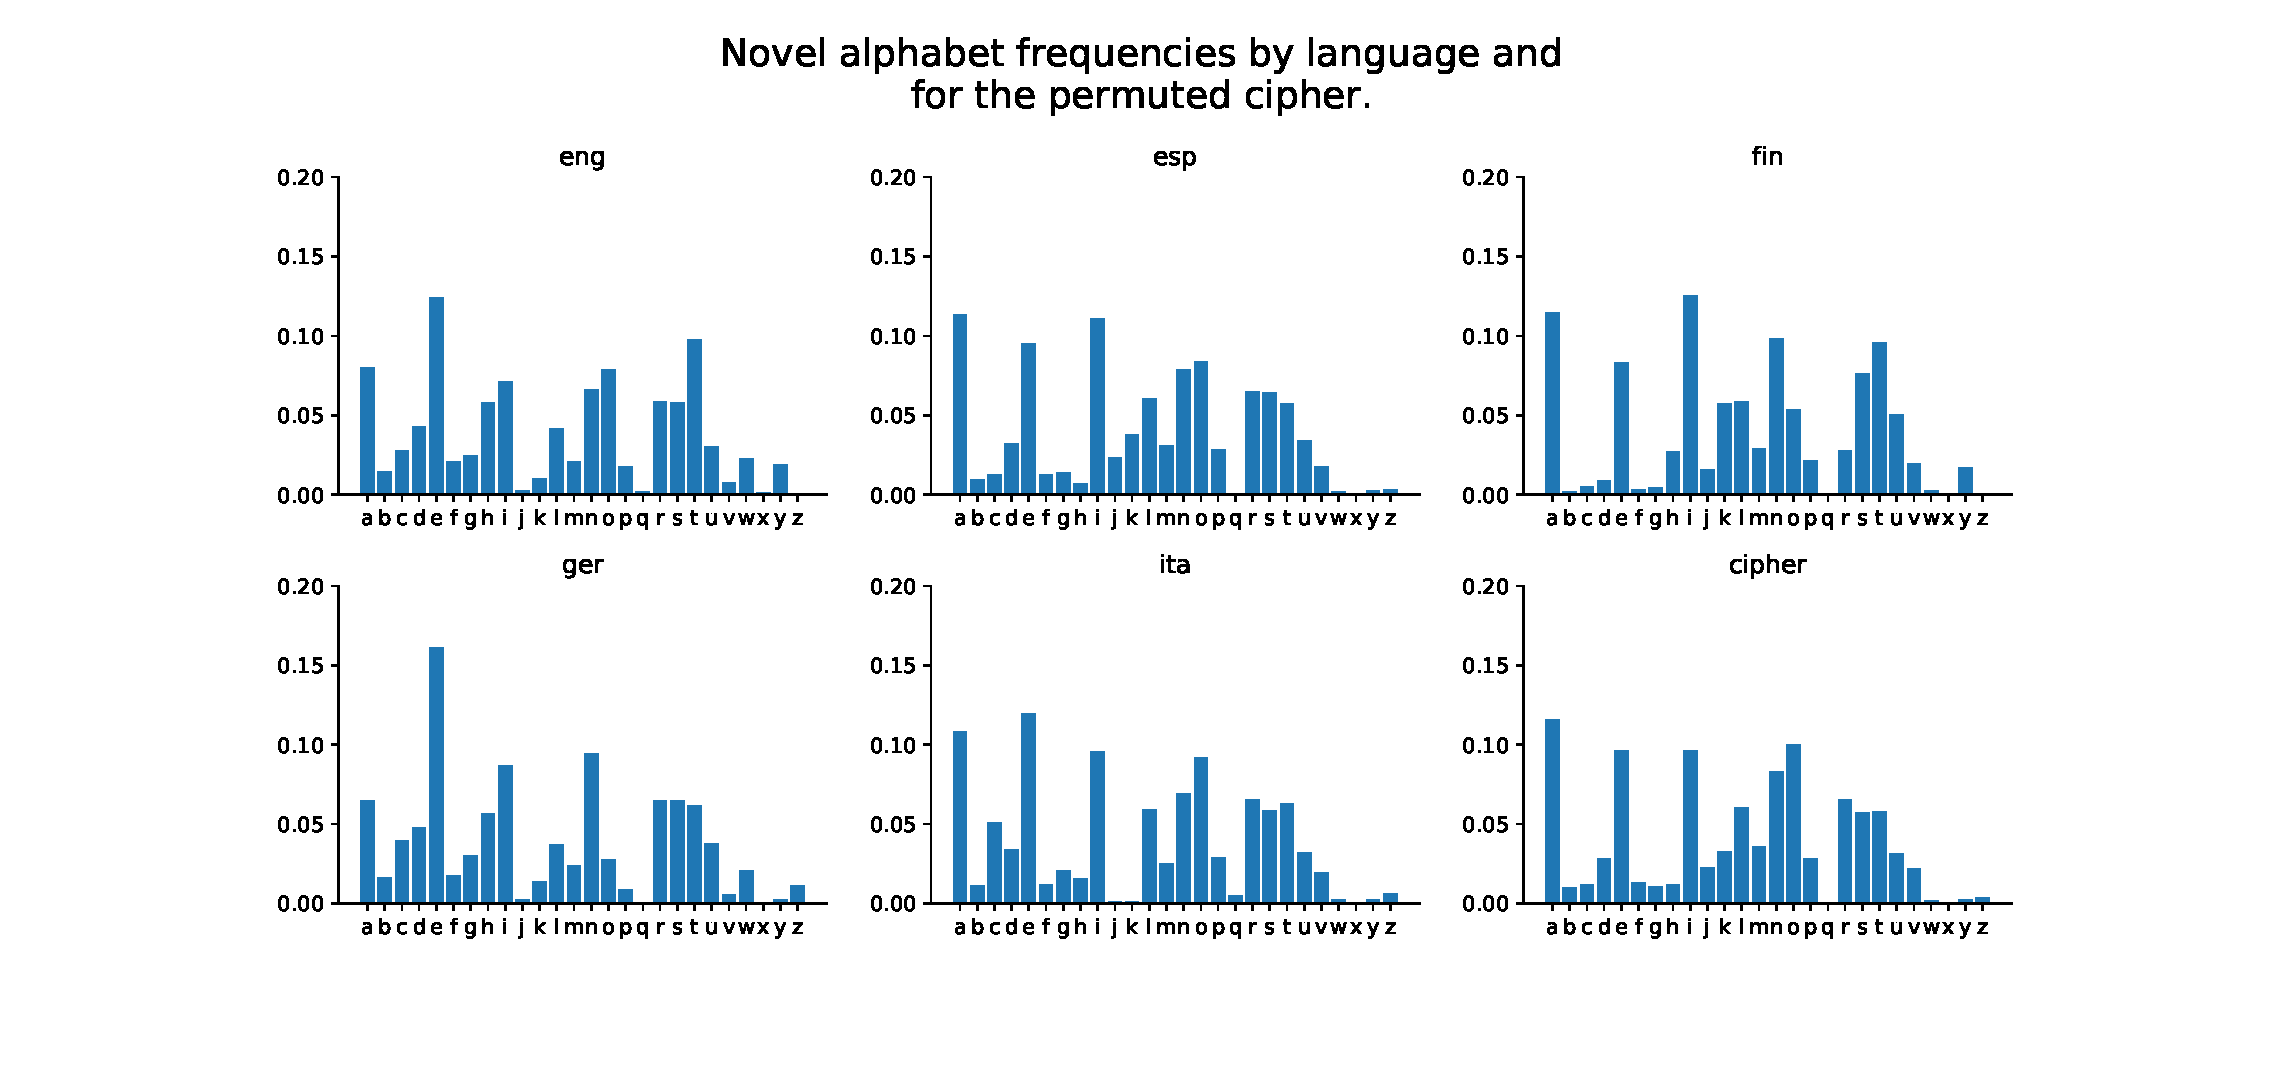
\includegraphics[width=1.3\textwidth]{assets/relative-freq.eps}}%
    \caption{Relative frequencies of the 6 provided inputs.}
    \label{fig:relfreq}
\end{figure}

To sanity check, we tested the properties of such distance, such as identity of indiscernibles,
symmetry and subaddittivity.

We then computed all the possible combinations resulting in table \autoref{table:restable}:

% fin-ger     : 0.30
% eng-fin     : 0.26
% ger-cipher  : 0.24
% esp-ger     : 0.24
% fin-ita     : 0.24
% eng-cipher  : 0.21
% eng-esp     : 0.21
% ger-ita     : 0.19
% fin-cipher  : 0.18
% esp-fin     : 0.16
% eng-ita     : 0.16
% eng-ger     : 0.14
% esp-ita     : 0.11
% ita-cipher  : 0.10
% esp-cipher  : 0.04

\begin{table}[H]
    \centering
    \begin{tabular}{c|c|c|c|c|c|c}\toprule[1.5pt]
    \backslashbox{P}{Q} & eng & esp & fin & ger & ita & cipher \\ \hline
        eng & 0 & 0.21 & 0.26 & 0.14 & 0.16 & 0.21 \\ \hline
        esp & 0.21 & 0 & 0.16 & 0.24 & 0.11 & 0.04 \\ \hline
        fin & 0.26 & 0.16 & 0 & 0.3 & 0.24 & 0.18 \\ \hline
        ger & 0.14 & 0.24 & 0.3 & 0 & 0.19 & 0.24 \\ \hline
        ita & 0.16 & 0.11 & 0.24 & 0.19 & 0 & 0.21 \\ \hline
        cipher & 0.21 & 0.04 & 0.18 & 0.24 & 0.21 & 0 \\\bottomrule[1.25pt]
    \end{tabular}
    \caption{Pairwise variational distance.}
    \label{table:restable}
\end{table}

If we exclude the cipher from our results, we have that the highest variational distance is between \textit{fin-ger} with a distance of $0.3$ while the lowest is between \textit{esp-ita} with a distance of $0.11$.

\end{solution}

\begin{subproblem}{2}
Compute the five collision probabilities $Coll(P_{\lang})$ for  $\lang \in \{ \textrm{eng, ger, esp, ita, fin} \}$.

\textbf{Note:} You do not have to submit your code.
\end{subproblem}
\begin{solution}
% Collision probabilities:
% fin     : 0.07674919239984539
% ger     : 0.07249092263220734
% ita     : 0.07128790076508662
% cipher  : 0.07008295280317041
% esp     : 0.06994154478831635
% eng     : 0.06554726160032555

\begin{table}[H]
\centering
\vspace{-2ex}
\begin{tabular}{ccccccc}\toprule[1.5pt]
\textit{l} & fin & ger & ita & cipher & esp & eng \\ \midrule
$\operatorname{Call}(P)$  & 0.076 & 0.072 & 0.071 & 0.070 & 0.069 & 0.065\\
\bottomrule[1.25pt]
\end{tabular}
\caption{Collision probabilities.}
\label{table:cprob}
\end{table}

The collision probabilities were calculated from the previous relative frequencies.


\end{solution}

\begin{subproblem}{1}
 Why is it called collision probability?
\end{subproblem}
\begin{solution}
It's called collision probability because it represents the probability that two independent
samples of random variables $X_1$, $X_2$ being sampled from the same distribution have of resulting
in equal values.
\end{solution}

\begin{subproblem}{2}
  You are \href{https://github.com/cschaffner/InformationTheory/blob/master/Problems/HW1/permuted_cipher.txt}{given the file} {\texttt{permuted\_cipher.txt}} that has been encrypted by (first removing spaces and then) shuffling around the
characters (i.e.\ by applying a permutation cipher). Note that this kind of
encryption preserves the letter frequencies. Compute the frequency distribution
$P_{\textit{cipher}}$ and figure out which language the original text was by
picking the one that minimizes by the variational distance
$\| P_{\textit{cipher}} - P_{\lang}\|$ with $\lang \in \{
\textrm{eng, ger, esp, ita, fin} \}$ as above.

\textbf{Note:} You do not have to submit your code.
\end{subproblem}
\begin{solution}
The language that seems to minimize the variational distance with the cipher is \textit{esp} as shown
in \autoref{table:restable}.
\end{solution}

\begin{subproblem}{1}
Would you have picked the same language when comparing the collision probability $Coll(P_{\textit{cipher}})$ to the ones above?
\end{subproblem}
\begin{solution}
Yes, as the distribution having the most similar collision probability with \textit{cipher} is indeed \textit{esp}.
\end{solution}

\end{nproblem}




%Entropy diagram for two variables:
%\begin{center}
%% the optional argument in [] lets you determine the size of the circles
%\entropydiagramXY[2]{$H(X)$}{$H(Y)$}{$H(XY)$}{$H(X|Y)$}{$H(Y|X)$}{$I(X;Y)$}
%\end{center}

\end{document}
\documentclass[a4paper,10pt]{article}
\usepackage{epsfig}
\usepackage{float}
\usepackage{slashbox}
\usepackage{wrapfig}
\usepackage{tabularx,ragged2e,booktabs,caption}
\usepackage{solutions}
\usepackage{amsmath,amssymb}
\DeclareRobustCommand{\bbone}{\text{\usefont{U}{bbold}{m}{n}1}}
\DeclareMathOperator{\EX}{\mathbb{E}}% expected value
\begin{document}
%%% fill in your team name and each student's name:
\frontpage{Hadamard}{Leonardo Romor, Maurice Frank, Simone Astarita, XinYu Fu, Yije Zhang}{1}

%%%%%%%%%%%%%%%%%%%%%%%%%%%%%%%%%%%%%%%%%%%%%%%%%%%%%%%%%%%%%%%%%%%%%%%%%%

\begin{nproblem}{7}{Two coins and a die}
You have two (fair) coins and a (fair) 4-sided die with outcomes $\{1,2,3,4\}$. Let $X$ be the number of heads after flipping the two coins and let $Y$ be the result of rolling the die. Let $Z$ be the average of $X$ and $Y$.
\end{nproblem}

\begin{subproblem}{2}
What is the distribution $P_Z$ of $Z$?
\end{subproblem}

\begin{solution}
We can first write down $P_X$ in \autoref{table:1} and $P_Y$ in \autoref{table:2}. Then, it is easy to get the distribution of $Z$ by simple counting. $P_Z$ is shown in \autoref{table:3}.

\begin{table}[ht]
\centering
\caption{Distribution of $X$}
\begin{tabular}{c c c c}
\hline
$X$ & 0 & 1 & 2 \\ [0.5ex]
\hline
P($X$)& $\frac{1}{4}$ & $\frac{1}{2}$ & $\frac{1}{4}$ \\
\hline
\end{tabular}
\label{table:1}
\end{table}

\begin{table}[ht]
\caption{Distribution of $Y$}
\centering
\begin{tabular}{c c c c c}
\hline
$Y$ & 1 & 2 & 3 & 4 \\ [0.5ex]
\hline
P($Y$)& $\frac{1}{4}$ & $\frac{1}{4}$ & $\frac{1}{4}$ & $\frac{1}{4}$\\
\hline
\end{tabular}
\label{table:2}
\end{table}

\begin{table}[ht]
\caption{Distribution of $Z$}
\centering
\begin{tabular}{c c c c c c c}
\hline
$Z$ & $\frac{1}{2}$ & 1 & $\frac{3}{2}$ & 2 & $\frac{5}{2}$ & 3\\ [0.5ex]
\hline
P($Z$) & $\frac{1}{16}$ & $\frac{3}{16}$ & $\frac{1}{4}$ & $\frac{1}{4}$ & $\frac{3}{16}$ & $\frac{1}{16}$\\
\hline
\end{tabular}
\label{table:3}
\end{table}
\end{solution}


\begin{subproblem}{3}
Compute the variances of $X$, $Y$ and $Z$.
\end{subproblem}

\begin{solution}
Just apply the definition of variance, easy to get:
    \begin{align}
        \mathop{{}\mathbb{E}}(X) &= 0 \times \frac{1}{4} + 1 \times \frac{1}{2} + 2 \times \frac{1}{4} = 1\\
        Var(X) &= (0-1)^{2} \times \frac{1}{4} + (1-1)^{2} \times \frac{1}{2} + (2-1)^{2} \times \frac{1}{4} = \frac{1}{2}\\
        \mathop{{}\mathbb{E}}(Y) &= 1 \times \frac{1}{4} + 2 \times \frac{1}{4} + 3 \times \frac{1}{4} + 4 \times \frac{1}{4} = \frac{5}{2} \\
        Var(Y) &= (1-\frac{5}{2})^{2} \times \frac{1}{4} + (2-\frac{5}{2})^{2} \times \frac{1}{4} + (3-\frac{5}{2})^{2} \times \frac{1}{4} + (4-\frac{5}{2})^{2} \times \frac{1}{4} = \frac{5}{4} \\
        \mathop{{}\mathbb{E}}(Z) &= \frac{1}{2} \times \frac{1}{16} + 1 \times \frac{3}{16} + \frac{3}{2} \times \frac{1}{4} + 2 \times \frac{1}{4} + \frac{5}{2} \times \frac{3}{16} + 3 \times \frac{1}{16} = \frac{7}{4} \\
        Var(Z) &= (\frac{1}{2}-\frac{7}{4})^{2} \times \frac{1}{16} + (1-\frac{7}{4})^{2} \times \frac{3}{16} \\
        &+ (\frac{3}{2}-\frac{7}{4})^{2} \times \frac{1}{4} + (2-\frac{7}{4})^{2} \times \frac{1}{4} + (\frac{5}{2}-\frac{7}{4})^{2} \times \frac{3}{16} + (3-\frac{7}{4})^{2} \times \frac{1}{16}= \frac{7}{16}
    \end{align}
\end{solution}

\begin{subproblem}{2}
You play the following game. If $2X \ge Y$, you win $X^2$ euros and otherwise you lose 1 euro. What is your expected total gain or loss after playing this game $40$ times?
\end{subproblem}

\begin{solution}
Let's define a new random variable $A = 2X - Y$ for one round. Also, define the return function $f(A)$ on $A$ as:
\begin{align}
    f(a) =  \begin{cases}
                -1 & a < 0 \\
                X^2 & 0 \leq a
            \end{cases}
\end{align}
According to the question, the expectation $\mathbb{E}[f(A)]$ can be computed as:
    \begin{align}
        \mathbb{E}[f(A)] = \sum_a p(a) f(a) = P(A \ge 0) \cdot X^{2} + P(A < 0)\cdot(-1)
    \end{align}
where we have $P(A \ge 0)$ as:
    \begin{align}
        P(A \ge 0) = P(X=1)\cdot P(Y=1\ or\ 2 ) + P(X=2) = \frac{1}{4} + \frac{1}{4} = \frac{1}{2}
    \end{align}
and $P(A < 0)$ as:
    \begin{align}
        P(A < 0) = 1 - P(A \ge 0) = \frac{1}{2}
    \end{align}
so come back to the $\mathbb{E}[f(A)]$:
    \begin{align}
        \mathbb{E}[f(A)] = P(X=1,Y=1\ or\ 2) \cdot 1^{2} + P(X=2) \cdot (2)^{2}+P(A<0) \cdot (-1) = \frac{3}{4}
    \end{align}
Since in each round, the flipping of a dice and a coin is clearly independent of the flipping in last round, $\{A_i\}_{1}^{40}$ are i.i.d. random variables. Hence, the expected total gain or loss after playing this game 40 times is:
    \begin{align}
        \mathbb{E}[\sum_{i=1}^{40} f(A_i)]=\mathbb{E}[40 \cdot f(A)]= 40 \cdot \mathbb{E}[f(A)]=40\cdot\frac{3}{4}=30
    \end{align}
\end{solution}











%%%%%%%%%%%%%%%%%%%%%%%%%%%%%%%%%%%%%%%%%%%%%%%%%%%%%%%%%%%%%%%%%%%%%%%%%%

\begin{nproblem}{9}{Deriving the weak law of large numbers}
\end{nproblem}
	\begin{subproblem}{2} \textbf{(Markov's inequality)} For any real non-negative random variable $X$ and any $t > 0$, show that
	\[
	P[X \geq t] \leq \frac{\mathbb{E}[X]}{t}\, .
	\]
\end{subproblem}

\begin{solution}

Given indicator function:
$$tI_{x\ge t} \le X$$
when $x<t$, $tI_{x\ge t}=0 \le X$,
else when $x\ge t$, $tI_{x\ge t}=t \le X$

Get the expected value for left and right sides, we obtain:
$$t\EX(I_{x\ge t}) \le \EX(X)$$

Substitute $\EX(I_{x\ge t}) = P[X \geq t]$ and after items rearrangement, we obtain:
	\[
	P[X \geq t] \leq \frac{\mathbb{E}[X]}{t}\, .
	\]
\end{solution}

\begin{subproblem}{1}
	Exhibit a random variable (which can depend on $t$) that achieves this inequality with equality.
\end{subproblem}

\begin{solution}
Either $x=0$ or $t=0$
\end{solution}

\begin{subproblem}{3} \textbf{(Chebyshev's inequality)} Let $Y$ be a random variable with mean $\mu$ and variance $\sigma^2$. Show that for any $\varepsilon > 0$,
	\[
	P[|Y - \mu| \geq \varepsilon] \leq \frac{\sigma^2}{\varepsilon^2} \, .
	\]
	\textbf{Hint:} Define a random variable $X := (Y - \mu)^2$.
\end{subproblem}

\begin{solution}
We define a random variable \(X := {(Y-\mu)}^2\). Therefore:
\begin{align*}
    P[|Y-\mu| \geq \epsilon]
    &= P[{(Y-\mu)}^2 \geq \epsilon^2] \\
    &= P[X\geq \epsilon^2]\\
    \sigma^2
    &= \EX[{(y-\mu)}^2]\\
    &= \EX[X]\\
\end{align*}
Using now the Markov inequality with \(t=\epsilon^2\) we have:
\begin{align*}
    P[X\geq \epsilon^2] &\leq \frac{\EX[X]}{\epsilon^2}
\end{align*}
which proves the Chebyshev inequality.

\end{solution}

\begin{subproblem}{3} (The weak law of large numbers.) Let $Z_1, Z_2, ..., Z_n$ real i.i.d. random variables with mean $\mu = \mathbb{E}[Z_i]$ and variance $\sigma^2 = \mathbb{E}[(Z_i - \mu)^2] < \infty$. Define the random variables $S_n = \frac{1}{n} \sum_{i=1}^n Z_i$. Show that
	\[
	P[|S_n - \mu | \geq \varepsilon] \leq \frac{\sigma^2}{n\varepsilon^2}\, .
	\]
	Thus, $P[|S_n - \mu| \geq \varepsilon] \to 0$ as $n \to \infty$. This is known as the weak law of large numbers (which we will use heavily in Week 03).
\end{subproblem}

\begin{solution}

Given Chebyshev's inequality
	\[
	P[|S_n - \mu| \geq \varepsilon] \leq \frac{Var[S_n]}{\varepsilon^2} \, .
	\]

Substitute $$Var[S_n]=\frac{\sum_{i=1}^n Var[Z_i]}{n^2}=\frac{\sigma^2}{n}$$

We obtain the weak law of large numbers
	\[
	P[|S_n - \mu| \geq \varepsilon] \leq \frac{\sigma^2}{n\varepsilon^2} \, .
	\]
where $P[|S_n - \mu| \geq \varepsilon] \to 0$ as $n \to \infty$
\end{solution}












%%%%%%%%%%%%%%%%%%%%%%%%%%%%%%%%%%%%%%%%%%%%%%%%%%%%%%%%%%%%%%%%%%%%%%%%%%

\begin{nproblem}{3}{Multiple-choice test}
A multiple-choice exam has 4 choices for each question. A student has studied enough so that the probability she will know the answer to a question is 0.5, the probability that she will be able to eliminate one choice is 0.25, otherwise all 4 choices seem equally plausible. If she knows the answer she will get the question right. If not she has to guess from the 3 or 4 choices.

As the teacher you want the test to measure what the student knows. If the student answers a question correctly, what is the probability she knew the answer? Give your answer with three decimals of precision.


\begin{solution}
First we look at the probability of guessing a MC-question correctly. For a question with \(n\) answers we need the possible combinations of correct answers (\textit{multiple}):
\begin{align*}
    \sum_{i=1}^n {n\choose i} = 2^n - 1
\end{align*}
Making the probability of guessing correctly the reciprocal of that.

There are three paths to the correct solution: she knows the solution (\(\frac{1}{2}\)), she eliminated one solution and guessed (\(\frac{1}{4}\cdot\frac{1}{2^3 - 1}\)) or she completely guessed (\(\frac{1}{4}\cdot\frac{1}{2^4 - 1}\)).

Therefore the probability of she not guessing is:
\[
p(\text{knowledge}=\text{yes}|\text{answer}=\text{correct})
= \frac{\frac{1}{2}}{\frac{1}{2} + \frac{1}{28} + \frac{1}{60}} = \frac{105}{116} = 0.905 = 90.517\%
\]
\end{solution}
\end{nproblem}











%%%%%%%%%%%%%%%%%%%%%%%%%%%%%%%%%%%%%%%%%%%%%%%%%%%%%%%%%%%%%%%%%%%%%%%%%%


\newcommand{\lang}{\textit{lang}}
\newcommand{\coll}{\textit{coll}}

\begin{nproblem}{8}{Computing Variational Distance (programming)}
The \emph{total variation distance} between two probability distributions $P$ and $Q$
over the finite alphabet $\mathcal{X}$ is defined as
\begin{align*}
\| P - Q \| := \frac12 \sum_{x \in \mathcal{X} } | P(x) - Q(x) |
\end{align*}
This distance measure is symmetric, fulfills the triangle inequality and is normalized, i.e.\ it is 0 iff $P=Q$ and 1 iff $P$ and $Q$ have disjoint support.

The \emph{collision probability} of a distribution $P$ over finite alphabet $\mathcal{X}$ is defined as
\begin{align*}
Coll(P) := \sum_{x \in \mathcal{X}} P(x)^2
\end{align*}

In this exercise, we are going to analyze the letter frequencies of \emph{Alice in
  Wonderland} in five different languages: English, German, Esperanto,
Italian and Finnish. You can find all necessary files here: \url{https://github.com/cschaffner/InformationTheory/tree/master/Problems/HW1}. Hereby, we are going to consider only the 26 English letters (without space) and ignore that languages like German and Finnish have important other letters such as {\"a}, {\"o}, {\"u}.

For $\lang \in \{ \textrm{eng, ger, esp, ita, fin} \}$, let $P_{\lang}$ be the frequency distribution of the 26 English letters (without space) of Alice in Wonderland.

\begin{subproblem}{2}
Compute all pairwise variational distances $\| P_{\lang} - P_{\lang'} \|$ for $\lang \neq \lang' \in \{ \textrm{eng, ger, esp, ita, fin} \}$. Which two languages are closest, which two are furthest apart in terms of variational distance?

\textbf{Note:} for this exercise and any future programming exercises, you do not have to submit your code. In the pdf that you hand in, describe in a few sentences which general strategy you used (e.g., what quantities did you compute and in what order?), any choices you made (e.g., how did you treat uppercase letters? How did you deal with edge cases?), and any `sanity check' computations you may have performed (e.g., did you check what the variational distance between a text file and itself was?) By adding this information, you may still receive partial credit for your approach, even if your final numerical answer is incorrect.
\end{subproblem}
\begin{solution}

To evaluate the \textit{variational distance} we performed some pre-processing
on the provided data.
First, we converted every uppercase letter in lowercase.
A second pass was done to remove any punctuation or special non ascii-lowercase
characters (26 characters "abcdefghijklmnopqrstuvwxyz"). This was
done by providing a translation table. After preparing the inputs we computed
the frequencies and relative frequencies treating them as the empirical probability
distributions of the alphabet.

In \autoref{fig:relfreq} the relative frequencies are shown.

\noindent
\begin{figure}[H]
    \centering
    \makebox[\textwidth][c]{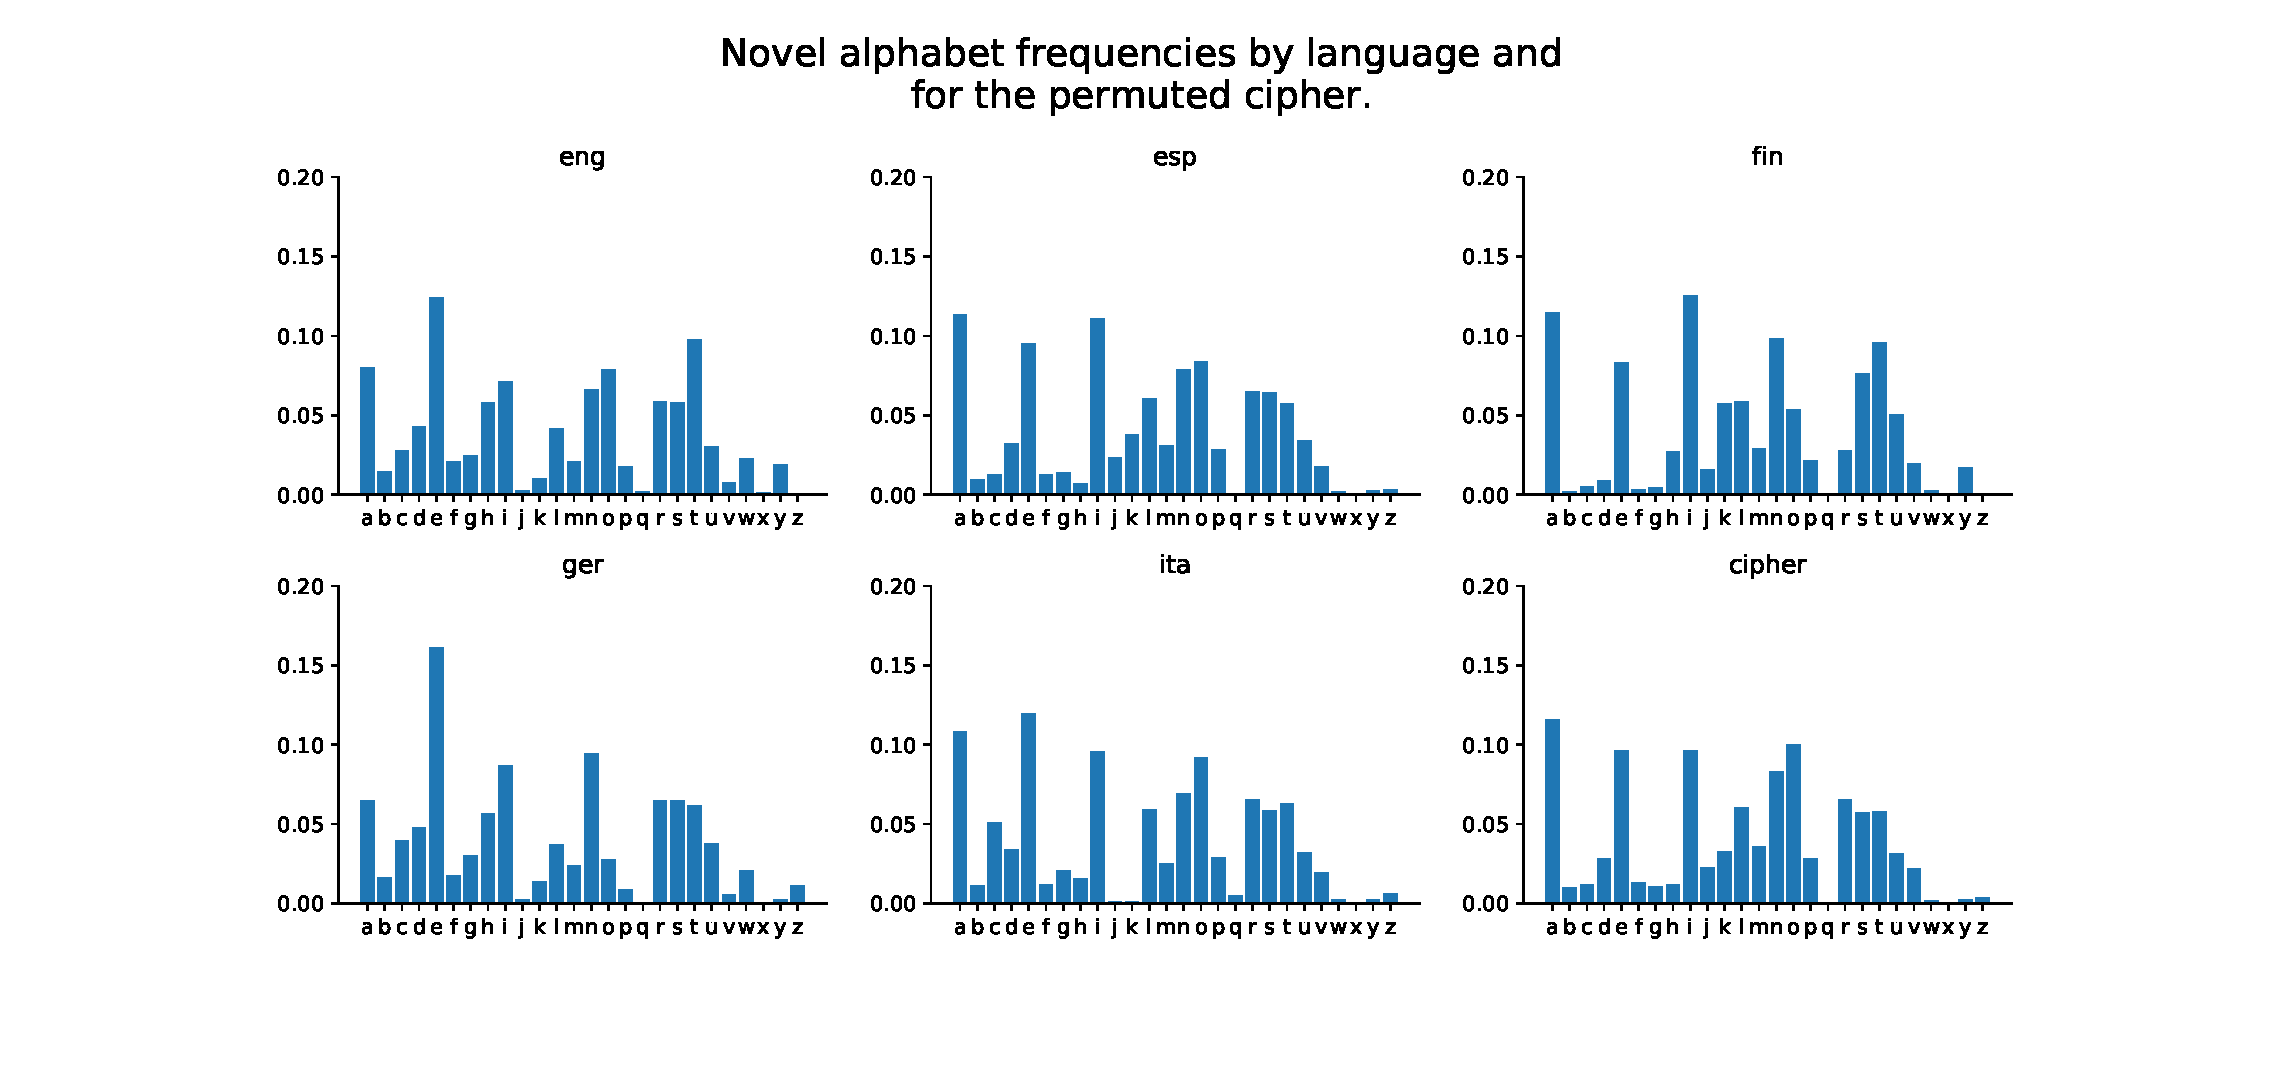
\includegraphics[width=1.3\textwidth]{assets/relative-freq.eps}}%
    \caption{Relative frequencies of the 6 provided inputs.}
    \label{fig:relfreq}
\end{figure}

To sanity check, we tested the properties of such distance, such as identity of indiscernibles,
symmetry and subaddittivity.

We then computed all the possible combinations resulting in table \autoref{table:restable}:

% fin-ger     : 0.30
% eng-fin     : 0.26
% ger-cipher  : 0.24
% esp-ger     : 0.24
% fin-ita     : 0.24
% eng-cipher  : 0.21
% eng-esp     : 0.21
% ger-ita     : 0.19
% fin-cipher  : 0.18
% esp-fin     : 0.16
% eng-ita     : 0.16
% eng-ger     : 0.14
% esp-ita     : 0.11
% ita-cipher  : 0.10
% esp-cipher  : 0.04

\begin{table}[H]
    \centering
    \begin{tabular}{c|c|c|c|c|c|c}\toprule[1.5pt]
    \backslashbox{P}{Q} & eng & esp & fin & ger & ita & cipher \\ \hline
        eng & 0 & 0.21 & 0.26 & 0.14 & 0.16 & 0.21 \\ \hline
        esp & 0.21 & 0 & 0.16 & 0.24 & 0.11 & 0.04 \\ \hline
        fin & 0.26 & 0.16 & 0 & 0.3 & 0.24 & 0.18 \\ \hline
        ger & 0.14 & 0.24 & 0.3 & 0 & 0.19 & 0.24 \\ \hline
        ita & 0.16 & 0.11 & 0.24 & 0.19 & 0 & 0.21 \\ \hline
        cipher & 0.21 & 0.04 & 0.18 & 0.24 & 0.21 & 0 \\\bottomrule[1.25pt]
    \end{tabular}
    \caption{Pairwise variational distance.}
    \label{table:restable}
\end{table}

If we exclude the cipher from our results, we have that the highest variational distance is between \textit{fin-ger} with a distance of $0.3$ while the lowest is between \textit{esp-ita} with a distance of $0.11$.

\end{solution}

\begin{subproblem}{2}
Compute the five collision probabilities $Coll(P_{\lang})$ for  $\lang \in \{ \textrm{eng, ger, esp, ita, fin} \}$.

\textbf{Note:} You do not have to submit your code.
\end{subproblem}
\begin{solution}
% Collision probabilities:
% fin     : 0.07674919239984539
% ger     : 0.07249092263220734
% ita     : 0.07128790076508662
% cipher  : 0.07008295280317041
% esp     : 0.06994154478831635
% eng     : 0.06554726160032555

\begin{table}[H]
\centering
\vspace{-2ex}
\begin{tabular}{ccccccc}\toprule[1.5pt]
\textit{l} & fin & ger & ita & cipher & esp & eng \\ \midrule
$\operatorname{Call}(P)$  & 0.076 & 0.072 & 0.071 & 0.070 & 0.069 & 0.065\\
\bottomrule[1.25pt]
\end{tabular}
\caption{Collision probabilities.}
\label{table:cprob}
\end{table}

The collision probabilities were calculated from the previous relative frequencies.


\end{solution}

\begin{subproblem}{1}
 Why is it called collision probability?
\end{subproblem}
\begin{solution}
It's called collision probability because it represents the probability that two independent
samples of random variables $X_1$, $X_2$ being sampled from the same distribution have of resulting
in equal values.
\end{solution}

\begin{subproblem}{2}
  You are \href{https://github.com/cschaffner/InformationTheory/blob/master/Problems/HW1/permuted_cipher.txt}{given the file} {\texttt{permuted\_cipher.txt}} that has been encrypted by (first removing spaces and then) shuffling around the
characters (i.e.\ by applying a permutation cipher). Note that this kind of
encryption preserves the letter frequencies. Compute the frequency distribution
$P_{\textit{cipher}}$ and figure out which language the original text was by
picking the one that minimizes by the variational distance
$\| P_{\textit{cipher}} - P_{\lang}\|$ with $\lang \in \{
\textrm{eng, ger, esp, ita, fin} \}$ as above.

\textbf{Note:} You do not have to submit your code.
\end{subproblem}
\begin{solution}
The language that seems to minimize the variational distance with the cipher is \textit{esp} as shown
in \autoref{table:restable}.
\end{solution}

\begin{subproblem}{1}
Would you have picked the same language when comparing the collision probability $Coll(P_{\textit{cipher}})$ to the ones above?
\end{subproblem}
\begin{solution}
Yes, as the distribution having the most similar collision probability with \textit{cipher} is indeed \textit{esp}.
\end{solution}

\end{nproblem}




%Entropy diagram for two variables:
%\begin{center}
%% the optional argument in [] lets you determine the size of the circles
%\entropydiagramXY[2]{$H(X)$}{$H(Y)$}{$H(XY)$}{$H(X|Y)$}{$H(Y|X)$}{$I(X;Y)$}
%\end{center}

\end{document}
